
\documentclass[]{./style/aiaa-tc}% insert '[draft]' option to show overfull boxes

\usepackage{./style/aiaa} %options in the preamble of the aiaa example.
\usepackage{./style/SU2style} % put the packages you might need here.
 \usepackage{subfigure}
 \usepackage{subfigmat}
 \usepackage{wrapfig}
 \usepackage{amsmath, texlogos}
 \usepackage{mathrsfs}
 \usepackage{color}
 \usepackage{epstopdf}
 \usepackage{epsfig}
 \usepackage{multirow}
 \usepackage{color}
 \usepackage{amsfonts}
 \usepackage{morefloats}
 \graphicspath{{fig/}}

% !TEX root = ../SU2-Scitech15.tex

\title{Residual and Grid Convergence of Compressible Turbulent Flows Using SU$^2$}

 \author{
     \ David E. Manosalvas\thanks{Ph.D. Candidate, Department of Aeronautics \& Astronautics, AIAA Student Member.},
     Francisco Palacios\thanks{Engineering Research Associate, Department of Aeronautics \& Astronautics, AIAA Senior Member.},
     \ Thomas D. Economon\thanks{Post-Doctoral Fellow in Aeronautics \& Astronautics, AIAA Member.},\\
     \ Heather Kline\thanks{Ph.D. Candidates (authors in alphabetical order), Department of Aeronautics \& Astronautics, AIAA Student Members.},
     \ Trent W. Lukaczyk\thanksibid{4},
     \ Kedar R. Naik\thanksibid{4}, 
     \ A. Santiago Padr\'on\thanksibid{4},\\
     \ Brendan Tracey\thanksibid{4},
     \ Anil Variyar\thanksibid{4},
     \ Andrew D. Wendorff\thanksibid{4},\\
   \ and Juan J. Alonso\thanks{Associate Professor, Department of Aeronautics \& Astronautics, AIAA Associate Fellow.}\\
  {\normalsize\itshape Stanford University, Stanford, CA, 94305, U.S.A.}
 }




\begin{document}

\maketitle

% !TEX root = ../SU2-Scitech15.tex
\begin{abstract}

One of the goals of the paper should be too provide the answers for CFD practitioners to questions such as: if I change this parameter what happens? Is the change big/small? how does it compare to changing other parameters?

\end{abstract}


%\printnomenclature % creates nomenclature section produced by MakeIndex
% I don't envision using a nomemclature.

% !TEX root = ../SU2-Scitech15.tex

\section{Introduction}
One of the advantages of using an implicit solver is the ability to choose higher Courant–Friedrichs–Lewy (CFL) numbers while maintaining stability. This feature allows for the use of local time stepping which translates into a faster rate of convergence by allowing each one of the cells to evolve at its maximum time stepping rate independently of the heterogeneity of the computational domain. This capability is particularly useful when dealing with Navier-Stokes simulations on which the cells used to model the boundary layer are significantly smaller than the cells representing the farfield. 

The most common initial condition when starting a fluid flow simulation is a uniform velocity distribution, and although it seams to make sense for cells away from the object of interest, it causes the generation of sharp gradients when significantly different size grids are located together and as well as within areas neighboring no-slip boundary condition point modeling walls. The non-physical transient collection of sharp gradients can cause the solver to diverge and the use of limiters are required to preserve stability. Ideally, in a well behaved subsonic problem the limiter will be active during the transient and will decrease its effect as the flow reached steady state~\cite{Venkatakrishnan:1993}.

For this study the NACA-0012 has been used, in addition to the wealth of experimental data that is available for this geometry, it is a canonical case in the development of numerical tools for the simulation of compressible flows, which makes it an important geometry to understand the limiter effects on the flow solution. To account for the effect that the grid resolution introduces, five different C-meshes have been used ranging from 3704 points (65 points in the airfoil surface) to 919424 points (1025 points in the airfoil surface). Particular emphasis has been put in the understanding of limiters with coarse meshes, in an effort to improve accuracy and reduce computational time reducing the cost of shape design optimization.

To be able to provide a background on the tools used within the SU$^2$ suite for this analysis, the paper has been divided as follows: ** Add the description of the sections as soon as we are done revising them **

% !TEX root = ../SU2-Scitech15.tex

\section{Physical Problem}

This is study we are simulating two-dimensional flow over a NACA 0012 airfoil under essentially incompressible free-stream conditions as specified by the AIAA Turbulence Model Benchmarking Working Group (TMBWG).  We are solving the Reynolds-averaged Navier-Stokes (RANS) equation. The S-A  turbulence models is used for all cases, and the free-stream conditions are shown in Table~\ref{tab:naca0012_runconditions}. 

\begin{wraptable}{r}{5.5cm}
  \begin{center}
  \begin{tabular}{||c|c||} \hline
    $M_\infty$ & $0.15$ \\ \hline 
    $Re_c$     & $6M$ \\ \hline
    $T_\infty$ & $300K$ \\ \hline
    $\alpha$ & $0^{\circ}$, $10^{\circ}$, $15^{\circ}$ \\ \hline
    $\mathcal{R}_{\tilde\nu}(U)$ & S-A \\ \hline
  \end{tabular}
  \caption{NACA 0012 free-stream conditions.} \label{tab:naca0012_runconditions}
  \end{center}
\end{wraptable} 

% !TEX root = ../SU2-Scitech15.tex

\subsection*{Reynolds-averaged Navier-Stokes (RANS) equations}
Describe the way the compressible RANS equations are being modeled 

\subsection*{Spalart-Allmaras Turbulence model}
Describe the way how the SA modeled is modeled


% !TEX root = ../SU2-Scitech15.tex

\subsection*{Numerical methods}
%Describe the numerical method used for the adventive fluxes,[x] the viscous fluxes[x] and the turbulence model. Highlight that all are 2nd order. Describe the time stepping scheme\cite{Palacios:2014,PalaciosEconomon:2014}.
In this section, the main numerical algorithms of SU2 will be described with a particular emphasis on the methods used to produce the results in this paper. The convective and viscous fluxes were calculated using a second-order Roe scheme. The S-A turbulence model was used, with variables convected using a second-order upwind method. Venkatakrishnan's limiter is used. Implicit local time-stepping is used to converge the problem to a steady-state solution, and the linear system is solved using the GMRES method with a maximum error tolerance of $\mathcal{O}(10^{-10})$ for each nonlinear iteration of the flow solver. LU-SGS preconditioning was used.

The limiter uses a tunable coefficient and a characteristic length. In this work the value of the limiter coefficient was varied between 0.1 and 10.0, along with variations in the CFL number to find appropriate values for each mesh. The limiter characteristic distance was chosen as 0.1 for the mesh with 257 points on the surface based on the recommendations of Venkatakrishan\cite{Venkatakrishnan:1993}. This value was scaled for the other meshes based on the number of surface points. The characteristic distance using this method can be found using $\Delta x_{char} = 25.7 c  / n_p $, where $n_p$ is the number of points on the surface and $c$ is the chord length. 

\subsubsection*{Venkatakrishnan Second-Order Limiter}
Limiters were developed for unstructured grids by Barth and Jespersen\cite{barth1989}. A limiter scheme finds a value $\Phi_i$ that limits the gradient in the piecewise-linear reconstruction of the solution. Limiters reduce unwanted oscillations in the solution, however tuning is required to maintain convergence and accuracy. The second-order reconstruction is shown in Eq.~\ref{eq:LimitedReconstr}, where $\vec{x}_i$ is the reference location, $u_i$ is the pointwise value at $x_i$, and $U_i(x)$ is the reconstructed distribution within cell $i$.
\begin{equation}\label{eq:LimitedReconstr}
U_i(\vec{x}) = \bar{u}_i + \Phi_i \nabla u_i \cdot (\vec{x}-\vec{x}_i ), \Phi\in [0,1]
\end{equation}
In Eq.~\ref{eq:VenkatakrishnanLim}, from Venkatakrishnan\cite{Venkatakrishnan:1993}, $\Delta x$ is a characteristic length, $K$ is the tunable limiter coefficient, and $\epsilon^2 = (K\Delta x)^3$. $\Delta_-=U(x_{i+1/2})-u_i$ and $\Delta_+ = u_i^{max}-u_i$. 
\begin{equation}\label{eq:VenkatakrishnanLim}
\Phi_{i+1/2} = \frac{1}{\Delta_-}\left[ \frac{(\Delta_+^2+\epsilon^2)\Delta_-^2\Delta_-^2\Delta_+}{\Delta_+^2+2\Delta_-^2+\Delta_-\Delta_++\epsilon^2}\right]
\end{equation}
In smooth regions, where $\epsilon^2$ dominates,  $\Phi_{i+1/2}$ reduces to 1 and provides no limiting. This means that the limiting is effectively turned off or reduced in regions where it is not needed. 

%-----------------------------------------------------------
\subsubsection*{Spatial Integration via the Finite Volume Method}
%-----------------------------------------------------------

Partial Differential Equations (PDEs) in SU2 are discretized using a finite volume method~\cite{barth95, hirsch1984,quarteroni97, jameson01, leveque02, wesseling00, jameson:1995a, jameson:1995b, toro1999} with a standard edge-based structure on a dual grid with control volumes constructed using a median-dual, vertex-based scheme. Median-dual control volumes are formed by connecting the centroids, face, and edge-midpoints of all cells sharing the particular node. After integrating the governing equations over a control volume and applying the divergence theorem, the semi-discretized, integral form of a typical PDE (such as the RANS equations above) is given by,
\begin{equation} \label{eq:DiscretizedEq}
\int_{\Omega_i}{\frac{\partial{U}}{\partial{t}}}\,d\Omega + \sum_{j \in \mathcal{N}(i)}(\tilde{F}_{c_{ij}}+\tilde{F}_{v_{ij}})\Delta{S}_{ij} -Q|\Omega_i| = \int_{\Omega_i}{\frac{\partial{U}}{\partial{t}}}\,d\Omega + R_i(U) = 0,
\end{equation}
 
where $U$ is the vector of state variables, and $R_i(U)$ is the numerical residual representing the integration of the spatial terms. $\tilde{F}_{c_{ij}}$ and $\tilde{F}_{v_{ij}}$ are the projected numerical approximations of the convective and viscous fluxes, respectively, and $Q$ is a source term. $\Delta{S}_{ij}$ is the area of the face associated with the edge $ij$, $\Omega_i$ is the volume of the control volume, and $\mathcal{N}(i)$ is the set of neighboring nodes to node $i$.

The convective and viscous fluxes are evaluated at the midpoint of an edge. The numerical solver loops through all of the edges in the primal mesh in order to calculate these fluxes and then integrates them to evaluate the residual at every node in the numerical grid. The convective fluxes can be discretized using centered or upwind schemes in SU2. Several numerical schemes have been implemented (JST~\cite{jameson1981}, Roe~\cite{roe1981}, AUSM~\cite{liou93}, HLLC~\cite{toro1999}, Roe-Turkel~\cite{turkel_1}, to name a few), and the code architecture allows for the rapid implementation of new schemes. Limiters are available for use with higher-order reconstructions for the upwind convective schemes. In order to evaluate the viscous fluxes using a finite volume method, flow quantities and their first derivatives are required at the faces of the control volumes. The gradients of the flow variables are calculated using either a Green-Gauss or weighted least-squares method at all grid nodes and then averaged to obtain the gradients at the cell faces. Source terms are approximated using piecewise constant reconstruction within each of the finite volume cells.

\subsubsection*{Integration of convective fluxes}

The convective fluxes can be discretized using central or upwind methods in SU2. Several numerical schemes have been implemented (JST, Lax-Friedrich, Roe, AUSM, HLLC, Roe-Turkel), but this section will focus on the numerical schemes used for this study (Roe).

The flux-difference-splitting scheme by Roe~\cite{roe1981} evaluates the convective fluxes from flow quantities reconstructed separately on both sides of the face of the control volume from values at the surrounding nodes:
\begin{equation} \label{eq:roe}
\tilde{F}_{c_{ij}} = \tilde{F}(U_i, U_j) = \left(\frac{\vec{F}^c_i +\vec{F}^c_j}{2}\right)\cdot \vec{n}_{ij} - \frac{1}{2} P|\Lambda|P^{-1}(U_i - U_j), 
\end{equation}
where $\vec{n}_{ij}$ is the outward unit normal associated with the face between nodes $i$ and $j$, $U_i$ is the vector of the conserved variables at point $i$ and $\vec{F^c_i}$ is the convective flux at node $i$. $P$ is the matrix of eigenvectors of the flux Jacobian matrix, constructed using the Roe averaged variables and projected in the $\vec{n}_{ij}$ direction, and $|\Lambda|$ is a diagonal matrix with entries corresponding to the absolute value of the eigenvalues of the flux Jacobian matrix. This discretization is first-order accurate in space. Second-order accuracy is easily achieved via reconstruction of variables on the cell interfaces by using a Monotone Upstream-centered Schemes for Conservation Laws (MUSCL) approach~\cite{Leer1979} with gradient limitation.


\subsubsection*{Integration of viscous fluxes}

In order to evaluate the viscous fluxes using a finite volume method, flow quantities and their first derivatives are required at the faces of the control volumes. The values of the flow variables, including the velocity components, the dynamic viscosity $\mu$ and the heat conduction coefficient $k$, are averaged at the cell faces in SU2. 

The gradients of the flow variables are calculated using either a Green-Gauss or least-squares method at all grid nodes and then averaged to obtain the gradients at the cell faces. The following correction~\cite{weiss1997} is applied in order to reduce the truncation error of the scheme:
\begin{equation}
\nabla \phi \cdot \vec n = \frac{\phi_{j}-\phi_i}{|x_{j}-x_i|}\alpha_f + \frac{1}{2}(\nabla \phi|_i + \nabla \phi|_j)\cdot(\vec n-\alpha_f \vec s),
\end{equation}
where $\vec {n}$ is the face normal, $\vec s$ is the normalized vector connecting the cell centroid across the face, $|x_{j}-x_i|$ is the distance between node $i$ and $j$ and $\alpha _f$ is chosen to be the dot product $\alpha_f = \vec s\cdot \vec {n}$. Again, the gradients $\nabla \phi|_i$ at node $i$ are computed using either the Green-Gauss or least-squares theorems.

A Finite Element Method (FEM) is also available to numerically evaluate the Laplacian operator. Finite element methods are based upon approximations to a variational formulation of the problem. A variational formulation requires the introduction of a space of trial functions, $\mathcal{T}=\left\{V(t,\vec x)\right\}$, and a space of weighting functions, $\mathcal{W}=\left\{W(t,\vec x)\right\}$. The problem consists of finding $V(t,\vec x)$ in $\mathcal{T}$ satisfying the problem boundary conditions, such that
\begin{equation} \label{ere}
\int_{\Omega}{W^T\left( \nabla^2 V \right)\,d\Omega}=0.
\end{equation}

To produce an approximate solution to the variational problem, a grid of finite elements is constructed on the domain, $\Omega$. It will be assumed that the discretization employs $p$ nodes. Finite-dimensional subspaces $\mathcal{T}^{(p)}$ and $\mathcal{W}^{(p)}$ of the trial and weighting function spaces, respectively, are defined by
\begin{equation} \label{deefg}
\mathcal{T}^{(p)}=\left\{V^{(p)}(\vec x)\,|\,V^{(p)}=\sum^p_{J=1}{V_J N_J(\vec x)}\right\}, \; \mathcal{W}^{(p)}=\left\{W^{(p)}(\vec x)\,|\,W^{(p)}=\sum^p_{J=1}{a_J N_J(\vec x)}\right\},
\end{equation}
where $V_J$ is the value of $V^{(p)}$ at node $J$. On the other hand, $a_1, a_2, \ldots, a_p$ are constant and $N_J(\vec x)$ is the piecewise linear trial function associated with node $J$. We now apply the finite element approximation by discretizing the domain of the problem into elements and introducing functions which interpolate the solution over nodes that compose the elements. The Galerkin approximation is determined by applying the variational formulation of Eq.~\ref{ere} in the following form: find $V^{(p)}$ in $\mathcal{T}^{(p)}$, satisfying the problem boundary conditions, such that
\begin{equation} \label{asdf}
\int_{\Omega}{N^T_I \left(\nabla^2 V\right) \,d\Omega} = 0,
\end{equation}
for $I=1,2,...,p$. The form assumed for $V^{(p)}$ in Eq.~\ref{deefg} can now be inserted into the left hand side of Eq.~\ref{asdf} and the result can be written as
\begin{equation}
\int_{\Omega}{N^T_I \left(\sum^p_{J=1}V_J \nabla^2 N_J \right) \,d\Omega}=\sum^p_{J=1} V_J \left(\int_{\Omega}{N^T_I \nabla^2 N_J \,d\Omega}\right)=0.
\end{equation}
Applying the divergence theorem gives
\begin{equation}
\sum^p_{J=1}  V_J \left( \int_{\Gamma}{N^T_I\left( \nabla N_J\cdot \vec \nu \right)\,d\Gamma}- \int_{\Omega}{ \nabla N^T_I\cdot \nabla N_J\,d\Omega}\right)= 0,
\end{equation}
where $\vec \nu$ is the outward unit normal associated with the control volume surface and the boundary integral disappears unless we are computing a boundary element with non-homogeneous Neumann conditions ($I$ is an exterior node). The result at a typical interior node $I$ is
\begin{equation}
\sum_{E\in I}\sum_{J\in E} V_J\left ( \int_{\Omega_E}{ \nabla N^T_I\cdot \nabla N_J\,d\Omega}\right)=0,
\end{equation}
where the first summation extends over the elements $E$ in the numerical grid which contain node $I$ and the second summation extends over nodes $J$ of the elements $E$. $\Omega_E$ is the portion of $\Omega$ which is represented by element $E$.
%-----------------------------------------------------------
\subsubsection*{Source term integration}
%-----------------------------------------------------------
Source terms are approximated using piecewise constant reconstruction within each of the finite volume cells. The source terms plays a fundamental role in plasma simulations (chemical reactions), free-surface problems (gravity effects), or in the formulation of turbulence and transition models.

%-----------------------------------------------------------
\subsection*{Time integration for steady simulation}
%-----------------------------------------------------------
%\cite{Palacios:2014,PalaciosEconomon:2014}
It is well known that Eq.~\ref{eq:DiscretizedEq} has to be valid over the whole time interval, so one has to make the choice of evaluating $R_i(U)$ either at time $t^{n}$ (explicit methods) or $t^{n+1}$ (implicit methods). Focusing on the implicit integration (SU2 also has a Runge-Kutta explicit method), the easiest way to discretize the system is by using an implicit Euler scheme which can be written as
\begin{equation}
\int_{\Omega_i}{\frac{\partial{U}}{\partial{t}}}\,d\Omega + R_i(U) \approx |\Omega_i| \frac{\mathrm{d}U_i}{\mathrm{d}t} + R_i(U) = 0 \quad \rightarrow \quad \frac{|\Omega_i^n|}{\Delta t_i^n} \Delta U_i^n = - R_i(U^{n+1}),
\label{eq:Implicit_Euler}
\end{equation}
where $\Delta U_i^n = U_i^{n+1} - U_i^n$. However, the residuals at time $n+1$ are unknown, and linearization about $t^n$ is needed:
\begin{equation}
R_i(U^{n+1})  =  R_i(U^n) + \frac{\partial R_i (U^n)}{\partial t} \Delta t_i^n + \mathcal{O}(\Delta t^2) = R_i(U^n) + \sum_{j \in \mathcal{N}(i)} \frac{\partial R_i (U^n)}{\partial U_j} \Delta U_j^n + \mathcal{O}(\Delta t^2).
\end{equation}
Finally, the following linear system should be solved to find the solution update ($\Delta U_i^n$),
\begin{equation}\label{linear_system}
\left( \frac{|\Omega_i|}{\Delta t_i^n} \delta_{ij} + \frac{\partial R_i (U^n)}{\partial U_j} \right) \cdot \Delta U_j^n = -R_i(U^n),
\end{equation}
where if a flux $\tilde F_{ij}$ has a stencil of points $\{i, j\}$, then contributions are made to the Jacobian at four points:
\begin{equation}
\frac{\partial R}{\partial U} := \frac{\partial R}{\partial U} + \left[
\begin{array}{ccccc}
\ddots & & & & \\
 & \frac{\partial \tilde{F}_{ij}}{\partial U_i} & \cdots & \frac{\partial \tilde{F}_{ij}}{\partial U_j} & \\
 & \vdots & \ddots & \vdots & \\
 & -\frac{\partial \tilde{F}_{ij}}{\partial U_i} & \cdots & -\frac{\partial \tilde{F}_{ij}}{\partial U_j} & \\
 & & & & \ddots 
\end{array}
\right].
\end{equation}

Note that, despite implicit schemes being unconditionally stable in theory, a specific value of $\Delta t_i^n$ is needed to relax the problem. SU2 uses a local-time-stepping technique to accelerate convergence to a steady state. Local-time-stepping allows each cell in the mesh to advance at a different local time step. Calculation of the local time step requires the estimation of the eigenvalues and first-order approximations to the Jacobians at every node $i$ according to
\begin{equation}
\Delta t_i=N_{CFL} \min{\left(\frac{|\Omega_i|}{\lambda^{conv}_i},\frac{|\Omega_i|}{\lambda^{visc}_{i}}\right)},
\end{equation}
where $N_{CFL}$ is the Courant-Friedrichs-Lewy (CFL) number, $|\Omega_i|$ is the volume of the cell $i$ and $\lambda^{conv}_i$ is the integrated convective spectral radius~\cite{eliasson2002} computed as 
\begin{equation}
\lambda^{conv}_i=\sum_{j \in \mathcal{N}(i)}(|\vec u_{ij}\cdot\vec n_{ij}|+c_{ij})\Delta S,
\end{equation}
where $\vec u_{ij} = (\vec u_i + \vec u_j)/2$, and $c_{ij} = (c_i + c_j)/2$ denote the velocity and the speed of sound at the cell face. $\vec n_{ij}$ denotes the normal direction of the control surface and $\Delta S$, its area. On the other hand, the viscous spectral radius $\lambda^{visc}_{i}$ is computed as
\begin{equation}
\lambda^{visc}_{i} = \sum_{j \in \mathcal{N}(i)}C \frac{\mu_{ij}}{\rho_{ij}} S_{ij}^2,
\end{equation}
where $C$ is a constant, $\mu_{ij}$ is the sum of the laminar and eddy viscosities in a turbulent calculation and $\rho_{ij}$ is the density evaluated at the midpoint of the edge $ij$.



%-----------------------------------------------------------
\subsubsection*{Spalart-Allmaras (S-A) Model:}
%-----------------------------------------------------------
In the case of the one-equation Spalart-Allmaras~\cite{spalart1992} turbulence model, the turbulent viscosity is computed as
\begin{equation} \label{eq nutur}
\mu _{tur}=\rho \hat{\nu}f_{v1},\quad f_{v1}=\frac{\chi ^{3}}{\chi ^{3}+c_{v1}^{3}}\mbox{,}\quad \chi =\frac{%
\hat{\nu}}{\nu }\mbox{,}\quad \nu =\frac{\mu _{dyn}}{\rho }.
\end{equation}
The new variable $\hat \nu$ is obtained by solving a transport equation where the convective, viscous, and source terms are given as follows:
\begin{equation} \label{eq:tersa0}
\vec F^{c} =  \vec v\hat{\nu},\quad
\vec F^{v} =  - \frac{\nu +\hat{\nu}}{\sigma }\nabla\hat{\nu},\quad
Q =  c_{b1}\hat{S}\hat{\nu}-c_{w1}f_{w}\left( \frac{\hat{\nu}}{d_{S}}\right) ^{2}+\frac{c_{b2}}{\sigma } |\nabla \hat{\nu}|^{2},
\end{equation}
where the production term $\hat S$ is defined as $\hat{S} = |\vec \omega| +\frac{\hat{\nu}}{\kappa ^{2}d_{S}^{2}}f_{v2}$ , $\vec \omega= \nabla \times \vec v$ is the fluid vorticity, $d_{S}$ is the distance to the nearest wall, and $f_{v2}=1-\frac{\chi }{1+\chi f_{v1}}$. The function $f_{w}$ is computed as $f_{w}=g\left[ \frac{1+c_{w3}^{6}}{g^{6}+c_{w3}^{6}}\right] ^{1/6}$, where $g=r+c_{w2}(r^{6}-r)$ and $r=\frac{\hat{\nu}}{\hat{S}\kappa ^{2}d_{S}^{2}}$. Finally, the set of closure constants for the model is given by 
\begin{equation}
\sigma =2/3,\;  c_{b1}=0.1355,\; c_{b2}=0.622,\; \kappa =0.41, \;c_{w1}=\frac{c_{b1}}{\kappa^2}+\frac{1+c_{b2}}{\sigma}, \; c_{w2}=0.3, \; c_{w3}=2, \; c_{v1}=7.1. 
\end{equation}

The physical meaning of the far-field boundary condition for the turbulent viscosity is the imposition of some fraction of the laminar viscosity at the far-field. On viscous walls, $\hat{\nu}$ is set to zero, corresponding to the absence of turbulent eddies very near to the wall.

% !TEX root = ../SU2-Scitech15.tex

\subsection*{Linear Solver}
The linear solver used for the results presented here was General Minimum Residual (GMRES) with Lower-Upper Symmetric-Gauss-Seidel (LU-SGS). 


%Describe how the Generalized minimum residual (GMRES) works and the limits at which we are using it for this cases. Describe the use of the Lower-Upper Symmetric-Gauss-Seidel (LU-SGS).


The SU2 framework includes the implementation of several linear solvers for solving Eq.~\ref{linear_system}. Specifically, the following methods are available:
\begin{itemize}
\item The Lower-Upper Symmetric-Gauss-Seidel (LU-SGS) method~\cite{yoon88, jameson81b, jameson87}. This is a stationary iterative method that is based on a measurement of the error in the result (the residual) which is used to form a ``correction equation".
\item The Generalized Minimal Residual (GMRES) method~\cite{Saad:1986}, which approximates the solution by the vector in a Krylov subspace with minimal residual. The Arnoldi iteration is used to find this vector.
\item The Biconjugate Gradient Stabilized  (BiCGSTAB) method~\cite{Vorst1992}, also a Krylov subspace method. It is a variant of the biconjugate gradient method (BiCG) and has faster and smoother convergence properties than the original BiCG.
\end{itemize}


Due to the nature of most iterative methods/relaxation schemes, high-frequency errors are usually well damped, but low-frequency errors (global error spanning the larger solution domain) are less damped by the action of iterative methods that have a stencil with a local area of influence. To combat this, SU2 contains an agglomeration multigrid implementation that generates effective convergence at all length scales of a problem by employing a sequence of grids of varying resolution (SU2 can automatically generate the coarse grids from the provided fine grid at runtime). Simply stated, the main idea is to accelerate the convergence of the numerical solution of a set of equations by computing corrections to the fine-grid solutions on coarser grids and applying this idea recursively~\cite{jameson86, mavriplis1998, mavriplis1995, borzi-2003, palacios-2011}. 

Preconditioning is the application of a transformation to the original system that makes it more suitable for numerical solution~\cite{pierce-1997}.
% !TEX root = ../SU2-Scitech15.tex

\subsection*{Convergence Optimization}
Describe the process used to find the CFL number that will converge the solution in the least number of iterations, and how this is done for each of the limiters values.





Most of this information can be found in the previous SU$^2$ papers \cite{Palacios:2014,PalaciosEconomon:2014}
% !TEX root = ../SU2-Scitech15.tex


\section{Computational Domain}

For this paper, the simulations are run on a family of five structured meshes ranging from extremely coarse to fine. These are stated in table ~\ref{tab:naca0012_mesh}. As described in the AIAA Turbulence Model Resources online, the meshes are all C-meshes with the farfield located at a distance of 500 chord lengths from the airfoil.  The mesh spacing near the boundary in the wall normal direction meets the $y+<=1$ condition.

\begin{wraptable}{r}{5.5cm}
  \begin{center}
  \begin{tabular}{||c|c||} \hline
    $Mesh No.$ &  Mesh points\\ \hline \hline
    $G0$ &  113 X 33\\ \hline \hline
    $G1$ & 225 X 65 \\ \hline 
    $G2$     & 449 X 129 \\ \hline
    $G3$ & 897 X 257 \\ \hline
    $G4$ & 1793 X 513 \\ \hline
  \end{tabular}
  \caption{NACA 0012 meshs.} \label{tab:naca0012_mesh}
  \end{center}
\end{wraptable} 


Characteristic based farfield boundary conditions are applied to the outer boundary of the mesh and an adiabatic wall boundary condition is applied to the airfoil surface.






% !TEX root = ../SU2-Scitech15.tex

\section{Results}
The flow past a NACA 0012 has been modeled using each one of the 5 meshes described at $0^\circ$, $10^\circ$ and $15^\circ$ angles of attack. To better understand the effect that the grid has in the flow solution and integrated forces, the pressure coefficients (Cp) for all the angles of attack simulated modeled using a limiter value of 0.1 have been plotted in Figure~\ref{fig:cp_lim0.1}.

\begin{figure}[]
  \begin{subfigmatrix}{2}
    \subfigure[$0^\circ$ Angle of Attack.]{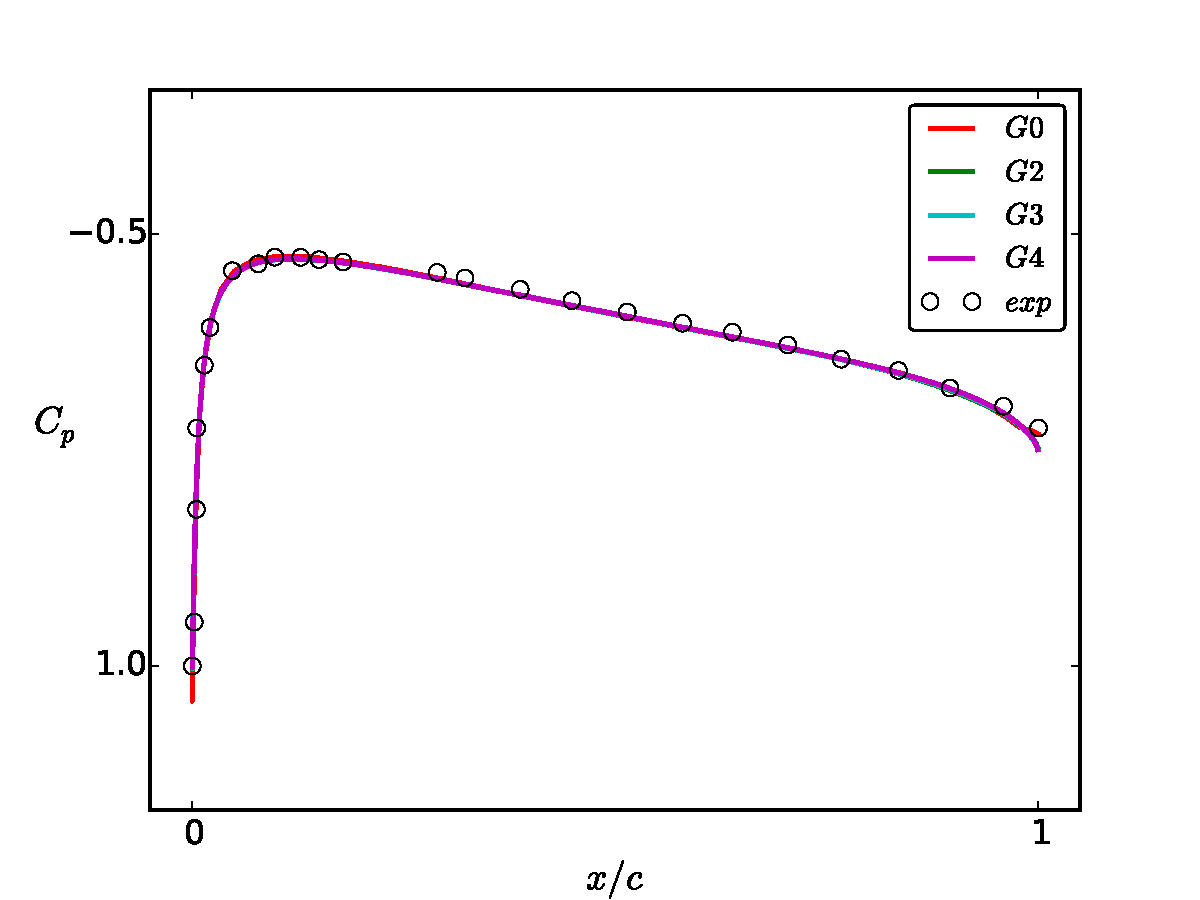
\includegraphics{Cp_vs_Grid_Lim_0_1_deg0.pdf}}
    \label{fig:cp_lim0.1_AoA0}
    \subfigure[$10^\circ$ Angle of Attack.]{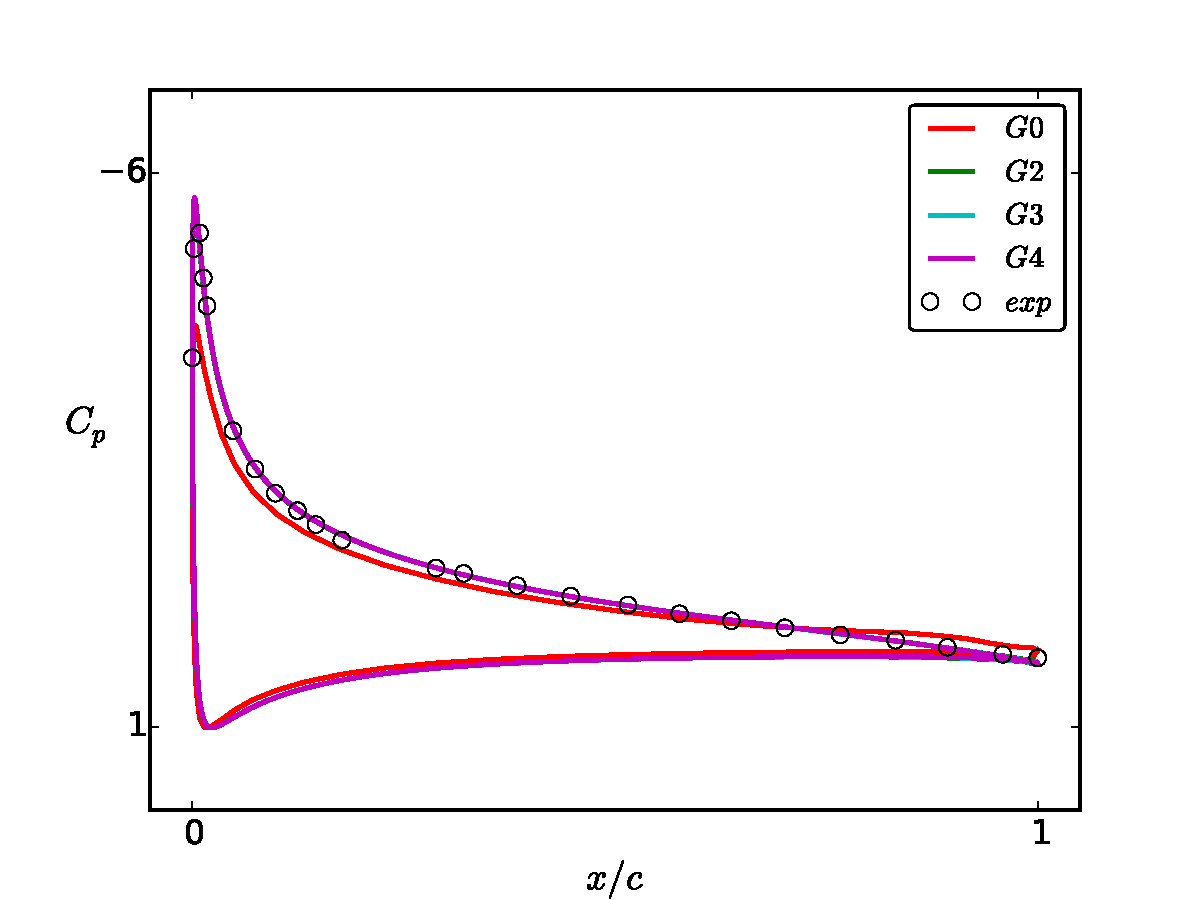
\includegraphics{Cp_vs_Grid_Lim_0_1_deg10.pdf}}
    \label{fig:cp_lim0.1_AoA10}
  \end{subfigmatrix}
  \begin{subfigmatrix}{1}
  	\subfigure[$15^\circ$ Angle of Attack.]{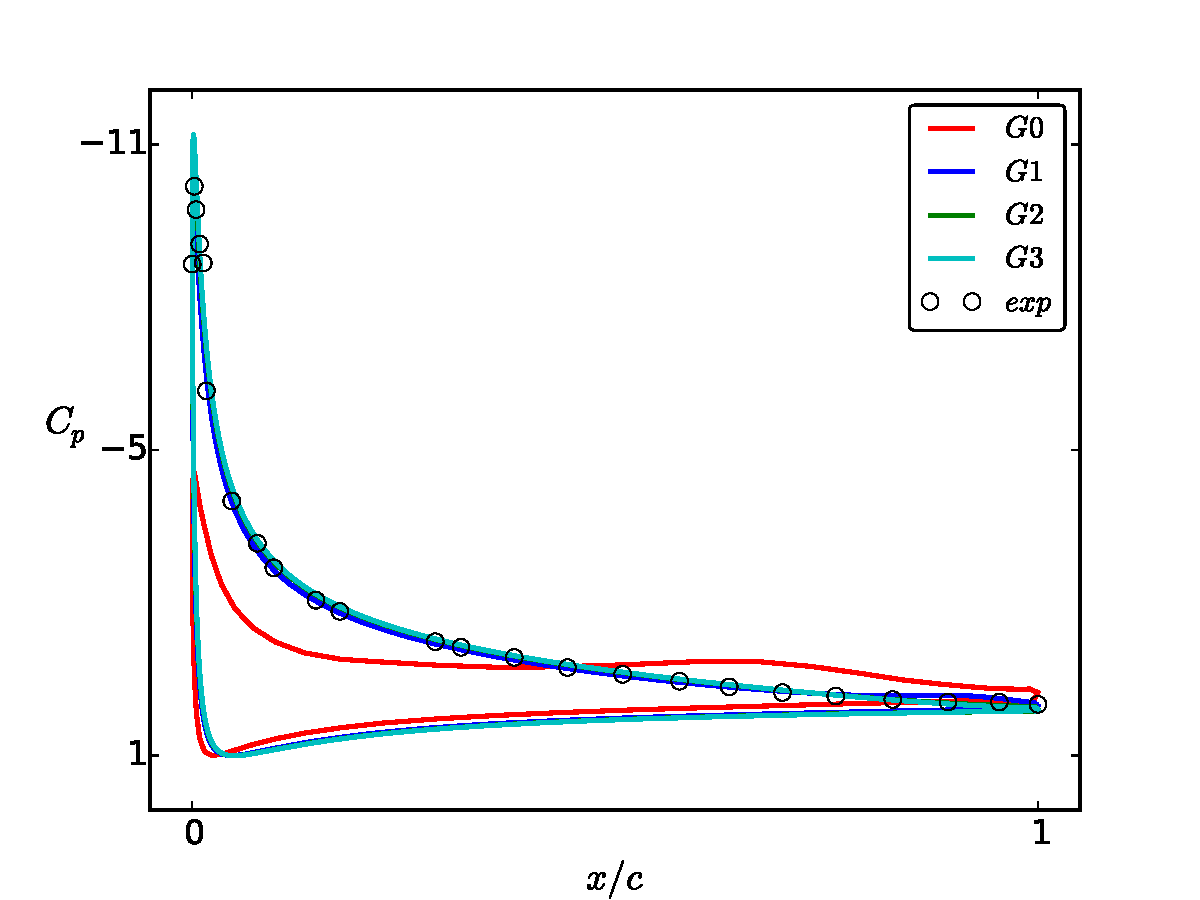
\includegraphics[width=.5\textwidth]{Cp_vs_Grid_Lim_0_1_deg15.pdf}}
    \label{fig:cp_lim0.1_AoA15}
  \end{subfigmatrix}
  
  \caption{Pressure coefficient of the NACA 0012 with a limiter value of 0.1 for 5 different grids.}
  \label{fig:cp_lim0.1}
\end{figure}

As can be expected, the Cp reflects that as the grid resolution increases Cp converges towards the experimental results. This behavior can be attributed to the lack of resolution mainly in the leading and trailing edges of the airfoil causing the miss prediction of the gradients and the flow structure.

Although it can be seen the that to achieve the correct solution, meshes such as G3 and G4 are adequate, there is a significant computational cost that has to be considered due to the high resolution involved. Keeping in mind the objective of this article to explore different alternatives to make the use of coarser grids for design purposes, various limiter values have been explored. 

\begin{figure}[]
  \begin{subfigmatrix}{2}
    \subfigure[$C_d$ Vs. limiter at $0^\circ$ Angle of Attack.]{\includegraphics{limiter_vs_drag_0deg.pdf}}
    \label{fig:lim_drag_AoA0}
    \subfigure[$C_l$ Vs. limiter at $0^\circ$ Angle of Attack.]{\includegraphics{limiter_vs_lift_0deg.pdf}}
    \label{fig:lim_lift_AoA0}
  \end{subfigmatrix}
  \begin{subfigmatrix}{2}
      \subfigure[$C_d$ Vs. limiter at $10^\circ$ Angle of Attack.]{\includegraphics{limiter_vs_drag_10deg.pdf}}
      \label{fig:lim_drag_AoA10}
      \subfigure[$C_l$ Vs. limiter at $10^\circ$ Angle of Attack.]{\includegraphics{limiter_vs_lift_10deg.pdf}}
      \label{fig:lim_lift_AoA10}
    \end{subfigmatrix}
    \begin{subfigmatrix}{2}
        \subfigure[$C_d$ Vs. limiter at $15^\circ$ Angle of Attack.]{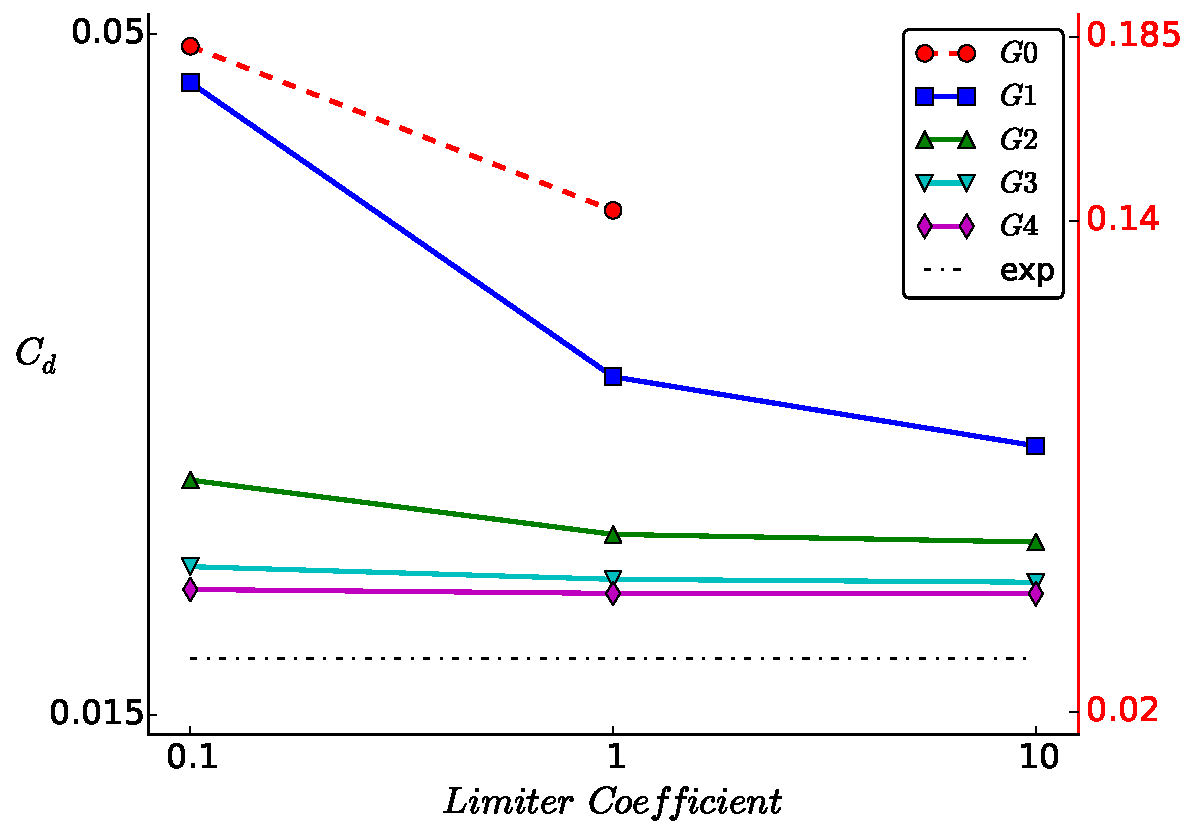
\includegraphics{limiter_vs_drag_15deg.pdf}}
        \label{fig:lim_drag_AoA15}
        \subfigure[$C_l$ Vs. limiter at $15^\circ$ Angle of Attack.]{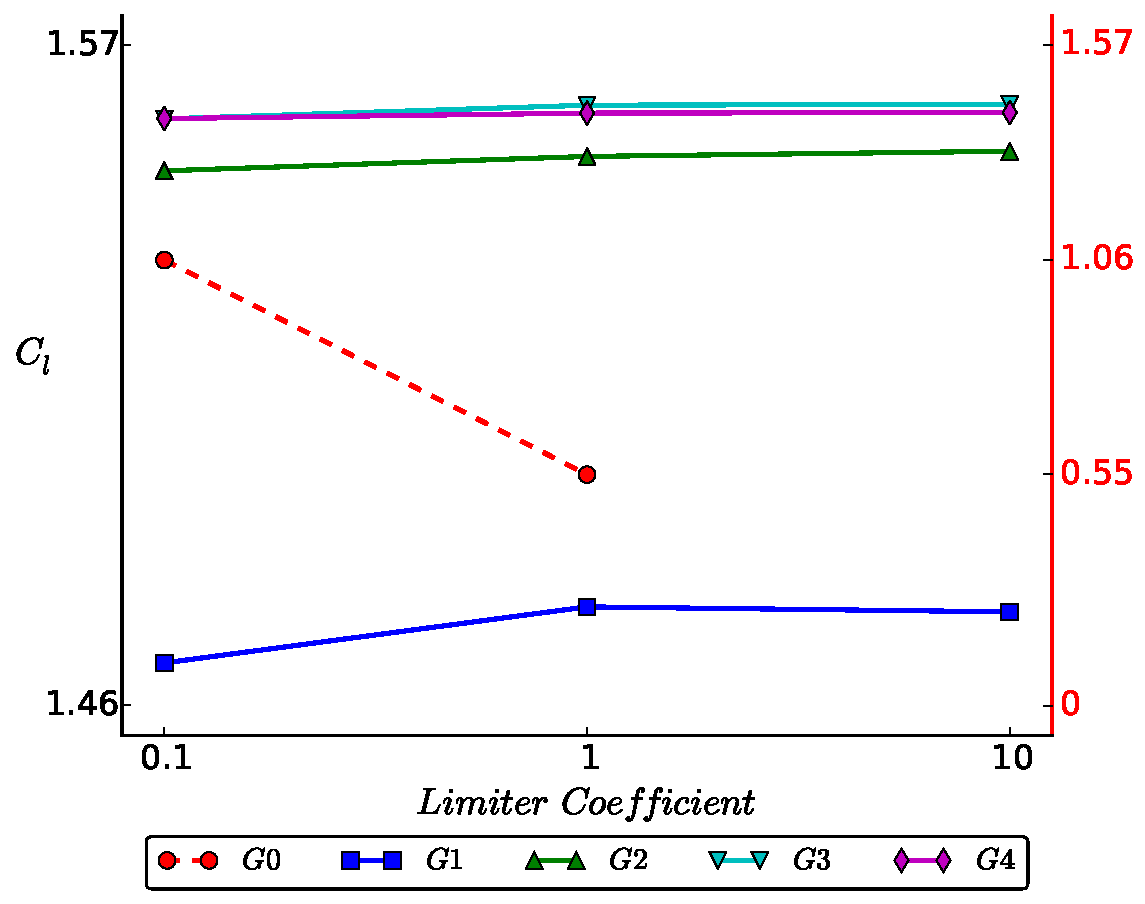
\includegraphics{limiter_vs_lift_15deg.pdf}}
        \label{fig:lim_lift_AoA15}
      \end{subfigmatrix}
  \caption{Relation between the limiter, grid resolution and integrated force coefficients for the NACA 0012. G0 results are displayed using the right hand side y-axis.}
  \label{fig:lim_grid}
\end{figure}

As can be seen from the Figure~\ref{fig:lim_grid}, the effect that the grid resolution in combination to the limiter value can be split into three categories. The first category is composed by G3 and G4, which are the finer grids and for which the limiter has little to no effect into the final converged solution. This results have been compared with available computational results and shown on Table~\ref{tab:naca_results} and are well within the range.

\begin{table}[]

  \begin{center}
  \begin{tabular}{c c c c c c c} \hline
  	\boldmath{$Contribution/Code$} & \boldmath{$C_l$}	& \boldmath{$C_l$} & \boldmath{$C_d$} & \boldmath{$C_d$} & \boldmath{$C_d$}     \\ 
  	 & \boldmath{$AoA=10$}	& \boldmath{$AoA=15$} & \boldmath{$AoA = 0$} & \boldmath{$AoA = 10$} & \boldmath{$AoA = 15$}     \\ \hline
  	
    $CFL3D$ & $1.0909$	& $1.5461$ & $0.00819$ & $0.01231$ & $0.02124$\\
    $FUN3D$ & $1.0983$	& $1.5547$ & $0.00812$ & $0.01242$ & $0.02159$\\
    $NTS$ 	& $1.0891$	& $1.5461$ & $0.00813$ & $0.01243$ & $0.02105$\\
    $JOE$ 	& $1.0918$	& $1.5490$ & $0.00812$ & $0.01245$ & $0.02148$\\
    $SUMB$  & $1.0904$	& $1.5446$ & $0.00813$ & $0.01233$ & $0.02141$\\
    $TURNS$ & $1.1000$	& $1.5642$ & $0.00813$ & $0.01233$ & $0.02140$\\
    $CGNS$  & $1.0941$	& $1.5576$ & $0.00817$ & $0.01225$ & $0.02073$\\
    $SU^2$  & $1.0988$	& $1.5577$ & $0.00801$ & $0.01277$ & $0.02264$\\
    $SU^2$ - $G4$ & $1.09644$	& $1.5578$ & $0.00810$ & $0.01236$ & $0.02146$\\
    
    
   	\hline
   	
  \end{tabular} 
  	\caption{Computational results for the NACA 0012 at RE = 6E6 and M = 0.15. $C_l$ os the lift coefficient, $C_d$ the drag coefficient and $AoA$ the angle of attack.}
  	\label{tab:naca_results}
  \end{center}
  \end{table}

The second section that comes out of the results represented on Figure~\ref{fig:lim_grid} is the middle grid range which is represented by G2. This is highly affected by the value of the limiter and as the limiter increases its effect is diminished, which allows the flow to converge towards the right solution. The upper limit of the limiter value is determined by the non-physical transient which takes place at the beginning of the simulation. The Cp plots of the NACA 0012 modeled by the G2 mesh at $15^\circ$ angle of attack are shown in Figure~\ref{fig:cp_vs_lim}. ** Describe the plots and how the higher the limiter value the closer it gets to the experimental data **

\begin{figure}[]
  \centering
    \includegraphics[width=0.5\textwidth]{Cp_vs_lim_gridG2_AOA15.pdf}
    \caption{Cp plots of the NACA 0012 represented by grid G2 at AoA = $15^\circ$.}
    \label{fig:cp_vs_lim}
\end{figure}

The third and final group that can be identified in Figure~\ref{fig:lim_grid} is composed by the coarse meshes G0 and G1 and care should be exercised when using them. The flow solutions obtained by using these meshes are highly dependent on the limiter value. It can be seen that as the limiter value increases, the integrated force coefficient approaches the expected solution, and to explore this trend further various limiter values were used and the results are shown in Figure~\ref{fig:limiter_exp}.

\begin{figure}[]
  \begin{subfigmatrix}{2}
    \subfigure[limiter Vs. $C_d$ for the G0 mesh.]{\includegraphics{limiter_vs_drag_15deg_G0.pdf}}
    \label{fig:lim_cd_AoA15_G0}
    \subfigure[limiter Vs. $C_l$ for the G0 mesh.]{\includegraphics{limiter_vs_lift_15deg_G0.pdf}}
    \label{fig:lim_cl_AoA15_G0}
  \end{subfigmatrix}
  \begin{subfigmatrix}{2}
  	\subfigure[limiter Vs. $C_d$ for the G1 mesh.]{\includegraphics[width=.5\textwidth]{limiter_vs_drag_15deg_G1.pdf}}
    \label{fig:lim_cd_AoA15_G1}
    \subfigure[limiter Vs. $C_l$ for the G1 mesh.]{\includegraphics[width=.5\textwidth]{limiter_vs_lift_15deg_G1.pdf}}
    \label{fig:lim_cl_AoA15_G1}
  \end{subfigmatrix}
  
  \caption{Limiter Vs Integrated force coefficients for the G0 and G1 meshes}
  \label{fig:limiter_exp}
\end{figure}

The G0 mesh is too coarse to be able to simulate the flow past a NACA 0012 accurately and, although the limiter has a big effect, its accuracy is limited by the mesh resolution. In the case of the G1, the integrated forces behave in a more favorable fashion and by choosing the limiter to be in the upper range, as can be seen in Figures~\ref{fig:lim_cd_AoA15_G1} and ~\ref{fig:lim_cl_AoA15_G1} one can potentially take advantage of the low computational cost while obtaining results that can be used at the first stages of shape design.

As can be clearly seen from the results show, the limiter plays a significant role in the behabior and final convergence value for coarse meshes, and to better understand the reason for this effect, the limiter value contour plot has been analyzed. 

\begin{figure}[]
  \begin{subfigmatrix}{2}
    \subfigure[G0 mesh.]{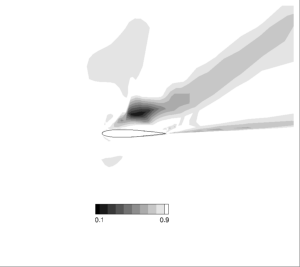
\includegraphics{lim_contour_Lim_0_1_deg15_GridG0.pdf}}
    \label{fig:contour_G0}
    \subfigure[G1 mesh.]{\includegraphics{lim_contour_Lim_0_1_deg15_GridG1.pdf}}
    \label{fig:contour_G1}
  \end{subfigmatrix}
  \begin{subfigmatrix}{1}
  	\subfigure[G2 mesh.]{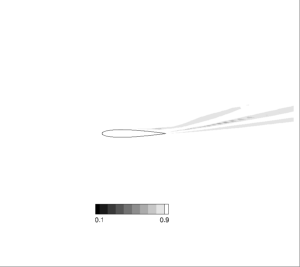
\includegraphics[width=.5\textwidth]{lim_contour_Lim_0_1_deg15_GridG2.pdf}}
    \label{fig:contour_G2}
  \end{subfigmatrix}
  
  \caption{Contour plot of the Venkatakrishnan limiter$\phi$ for flow at AoA = $15^\circ$ with a limiter value of 0.1. }
  \label{fig:limiter_contour}
\end{figure}

** Describe the results of this three plots and come to a conclusion on the main reason for the limiters effect **



% !TEX root = ../SU2-Scitech15.tex

\section{Conclusions}
Sum up what we have learned and correlations and conclusions found.





% !TEX root = ../SU2-Scitech15.tex

\section*{Acknowledgments}

Lets thank someone.



% !TEX root = ../SU2-Scitech15.tex

\bibliographystyle{aiaa}
\bibliography{../bib/}
%Local path to bibliography might not work.


\end{document}
